\clearpage
\onecolumngrid

\setcounter{figure}{0}
\renewcommand{\thefigure}{S\arabic{figure}}
\setcounter{section}{0}
\renewcommand{\thesection}{S\arabic{section}}
%%%%%%%%%%%%%%%%%%%%%%%%%%%%%%%%%%%%%%%%%%%%%
\begin{center}
  \textbf{\large Supplementary Material for Does Memory Burden Open\\ a New Mass Window for Primordial Black Holes as Dark Matter?}\\[.2cm]
  \vspace{0.05in}
  {Gabriele Montefalcone, Dan Hooper, Katherine Freese, Chris Kelso, Florian K{\"u}hnel, and Pearl Sandick}
\end{center}


%%%%%%%%%%%%%%%%%%%%%%%%%%%%%%%%%%%%%%%%%%%%%
\section{S1. Methodology}\label{sec:s1}
In Ref.~\cite{Kawasaki:2017bqm}, the authors employed a sophisticated code to study the effects of long-lived particles on the primordial light element abundances. These results were adapted in Ref.~\cite{Keith:2020jww} to derive constraints on the presence of PBHs, assuming their semi-classical evaporation.  In this \textit{letter}, we have followed this same procedure, modified to account for the effects of memory burden on the time and temperature profile of the Hawking radiation. 

For each set of parameters, we first derived a constraint based purely on the semi-classical phase of the black holes' evaporation (defined as the time window over which $M > q M_{i}$). Following Ref.~\cite{Keith:2020jww}, we found the time at which the median unit of energy (in the photodisassociation era of BBN, $T \lsim 0.4\,{\rm keV}$~\cite{Kawasaki:1994af}) or the median meson (in the hadrodisassociation era, $T \gsim 0.4\,{\rm keV}$) is produced through black hole evaporation, and then mapped this result onto the corresponding lifetime of a decaying particle~\cite{Kawasaki:1994af}. We further calculated the average energy of the particles that were radiated from the black holes during this period and mapped this result onto a mass for the corresponding decaying particle species. 

For black holes in the memory-burdened phase, we have mapped the time ane temperature profile onto that of a decaying particle species with a lifetime, $\tau$, in the range of $10 \times t_{\rm MB}$ and $10^{-3} \times t_{\rm evap}$, where $t_{\rm MB}$ is the time at which $M=q M_{i}$. For each lifetime, we calculated the total energy radiated from black holes between $t= 10^{-3}\,\tau$ and $10^{2}\,\tau$. If this weighted quantity of energy injection exceeded the constraints presented in Refs.~\cite{Keith:2020jww, Kawasaki:2017bqm} for any of the lifetimes in the stated range, we consider the scenario in question to be ruled out. Note that we have taken the temperature of the black hole to be constant during the memory-burdened phase, with $T_{\rm BH} = M^{2}_{\rm Pl}/(8 \pi q M_{i})$.

To derive constraints based on the CMB, we have made use the results presented in Ref.~\cite{Acharya:2019uba}, which considered the case of decaying particles (see also, Refs.~\cite{Slatyer:2016qyl, Poulin:2016anj}). We applied these results in close analogy to how we applied the results of Refs.~\cite{Keith:2020jww,Kawasaki:2017bqm}, again modifying the approach to account for the effects of memory burden on the time and temperature profiles of black hole evaporation. Note that the constraints from the CMB are largely insensitive to the mass of the decaying particle species~\cite{Slatyer:2016qyl}, so we simplified our procedure by taking the weakest constraint from Fig.~9 of Ref.~\cite{Acharya:2019uba}, regardless of the black hole's temperature. This approximation is conservative and in some cases could potentially weaken our constraints by as much as an order of magnitude. 



%%%%%%%%%%%%%%%%%%%%%%%%%%%%%%%%%%%%%%%%%%%%%
\section{S2. Results for Other Choices of $q$, $\delta$, and $k$}\label{sec:s2}

\begin{figure}
\vspace{-.5cm}
    \centering
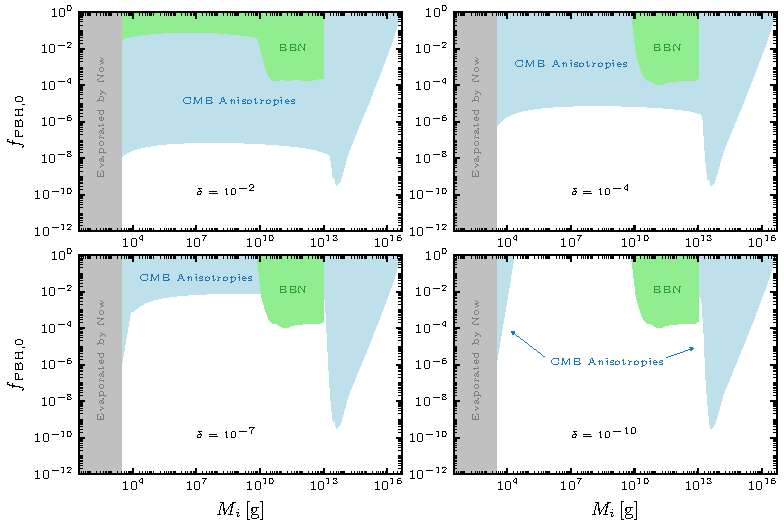
\includegraphics[width=1\linewidth]{letter_figures/fXfEM_combined_constraints_varying_delta_v1.pdf}
    \caption{Upper limits on the abundance of primordial black holes as a function of their initial mass, shown for four small values of $\delta$. In the limit $\delta\rightarrow 0$, we recover the results of the step-like memory burden approximation. Constraints are derived from both the primordial light element abundances (green) and CMB anisotropies (blue), highlighting how a continuous transition to the memory-burden phase affects these bounds. The gray region corresponds to primordial black holes that would have fully evaporated within the age of the Universe. Here, we have adopted $q=0.8$ and $k=2$, with $f_{{\rm PBH},0}$ denoting the initial fraction of the dark matter that consists
of primordial black holes.}
    \label{fig:results_3}
\end{figure}

In the main body of this \textit{letter}, we presented results for a small selection of $q$ and $\delta$. Here, we show results for other choices of these parameters. In Fig.~\ref{fig:results_3}, our constraints are given for the case of $q=0.8$ and $k=2$, and for four small values of $\delta$. In the limit of $\delta \rightarrow 0$, we recover the results of the step-like approximation. 

\begin{figure}
    \centering
    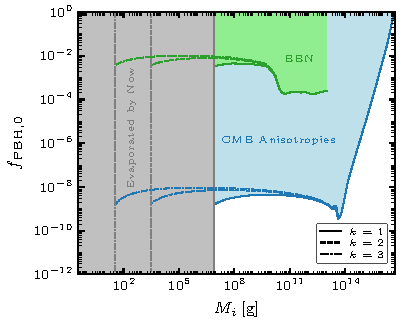
\includegraphics[width=.5\linewidth, height=0.416666\linewidth]{letter_figures/fXfEM_combined_constraints_varying_k_v1.pdf}
    \caption{As in Fig.~\ref{fig:results_3}, but for three values of $k$. From this comparison, we see that this parameter choice has little impact on the resulting bounds.  Here, we have adopted $q=0.8$ and $\delta=0.1$.}
    \label{fig:results_4}
\end{figure}

Throughout this \textit{letter}, we have adopted $k=2$, as suggested by numerical studies~\cite{Dvali:2020wft}. In Fig.~\ref{fig:results_4}, we compare these results to those obtained for $k=1$ and $k=3$. From this, we see that this parameter has little impact on our constraints.



%%%%%%%%%%%%%%%%%%%%%%%%%%%%%%%%%%%%%%%%%%%%%
\section{S3. Early Onset Memory Burden}\label{sec:s3}

If the parameter, $q$, is sufficiently close to unity, black holes will end their semi-classical phase after losing only a tiny fraction of their initial mass, becoming quickly stabilized by the memory-burden effect. If this is the case, then the constraints from BBN and the CMB will be much weaker than what we have found in the case of $q\sim 0.1-0.9$.

We illustrate this in Fig.~\ref{fig:results_2}, where we plot the constraints on PBHs for four small values of $(1-q)$. Here, we have adopted $k=2$ and $\delta/(1-q) =0.1$. Only for $(1-q) \lsim 10^{-10}$ does the effect of memory burden open a new mass window for PBHs to make up the dark matter of our Universe.  

\begin{figure}
    \centering
    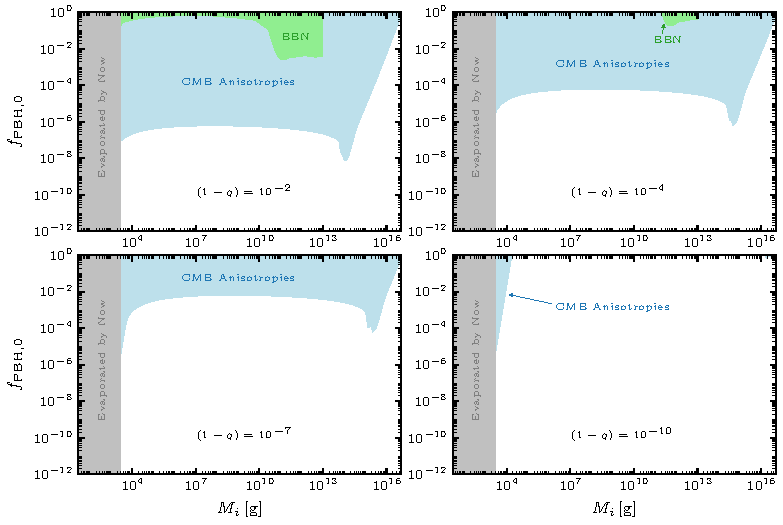
\includegraphics[width=1\linewidth]{letter_figures/fXfEM_combined_constraints_varying_1mq_v1.pdf}
    \caption{As in Fig.~\ref{fig:results_3}, but for four small values of $(1-q)$. Here, we have adopted $k=2$ and $\delta/(1-q)=0.1$.  
    A new mass window over which primordial black holes can constitute the dark matter of our Universe appears only if  $(1-q) \lsim 10^{-10}$.}
    \label{fig:results_2}
\end{figure}